\documentclass[conference]{IEEEtran}
%\documentclass[sigconf]{acmart}
\makeatletter
\def\ps@headings{%
\def\@oddhead{\mbox{}\scriptsize\rightmark \hfil \thepage}%
\def\@evenhead{\scriptsize\thepage \hfil \leftmark\mbox{}}%
\def\@oddfoot{}%
\def\@evenfoot{}}
\makeatother
\pagestyle{empty}
\usepackage[document]{ragged2e}
\usepackage{url}
\usepackage{graphicx,subfigure}
\usepackage{epstopdf}
\usepackage{amsmath}
\usepackage{algorithm}
\usepackage{algpseudocode}
\usepackage{amsmath}
\usepackage{amssymb}
\usepackage{amsthm}
\usepackage{epsfig}
\newtheorem{theorem}{Theorem}
\renewcommand{\algorithmicrequire}{\textbf{Input:}} % Use Input in the format of Algorithm
\renewcommand{\algorithmicensure}{\textbf{Output:}} % Use Output in the format of Algorithm
\usepackage{amsfonts}
%\newtheorem{theorem}{Theorem}[section]
\newtheorem{mydef}{Definition}[section]
%\newtheorem{lemma}{Lemma}[section]
\usepackage{multirow}
\usepackage{color}
\usepackage{array}
\usepackage{listings}
\usepackage{hyperref}
\usepackage[underline=true]{pgf-umlsd}

\usepackage{graphicx}
\usepackage{subcaption}

\usepackage{graphicx,array,booktabs}
\newcolumntype{M}[1]{>{\centering\arraybackslash}m{#1}}

\newlength{\subfigwidth}
\setlength{\subfigwidth}{50mm}


\newcommand{\tabincell}[2]
{\begin{tabular}
		{@{}#1@{}}#2\end{tabular}}
\usepackage{setspace}
\renewcommand{\labelitemi}{$\vcenter{\hbox{\tiny$\bullet$}}$}


\hyphenation{op-tical net-works semi-conduc-tor}




\begin{document}
\graphicspath{{photos/},{../diagrams/}}



\title{Team 2 \linebreak
 Chicago Car Accidents Assessment Utilizing Clustering Analysis}

\author{\IEEEauthorblockN{1\textsuperscript{st} Hodgetts, Michael }
\IEEEauthorblockA{\textit{Electrical Engineering Dept} \\
\textit{EE-695 - Machine Learning }\\
Hoboken, NJ \\
mhodgetts@comcast.net}
\and
\IEEEauthorblockN{2\textsuperscript{nd} Paladugu, Rithvika}
\IEEEauthorblockA{\textit{Computer Engineering} \\
\textit{EE 695 - Machine Learning}\\
Hoboken, NJ \\
paldugurithvika@gmail.com}

}

\maketitle


\begin{abstract}
Practice as a team to analyse unsupervised data by exploring various clustering methods (k-means, k-modes, kprototype, Gaussian and DBSCAN) on Chicago Accident database.
\end{abstract}

\section{Introduction}
Utilizing two datasets from Chicago Department website (Crashes and People related to Crashes), we like to find areas/neighborhoods within the city that have different characteristics in terms of the attributes available.  Dataset is large (750K rows) so we decided to look at only 2 years, i.e. 2021 and 2022 which reduces the row count to about 250K.  There is a good amount of prep to get data suitable for cluster analysis (ETL, Hot Encoding, data cleanup)
We tried 5 different cluster methods with varying results.  We'll give some brief description of each method and its pros and cons for this particular data set.  We will illustrate some of the main differences these assigned clusters present. Provide a summary of each cluster characteristics to illustrate the main differences between them.  

Figure 1 illustrates Chicago Heatmap of Crashes by Zip code.  Hade to use partial data since the original data had no zip for the crashes so had to use Nomatin to extract in python but there a limitation on how many you can search without further payment.  You can see that the majority of the crashes are in the lower half of the city.

\begin{figure}[!h]
	\includegraphics[width=\linewidth]{Zip_pop_map.png}
	\caption{Chicago Heatmap for Crashes by Zipcode}
	\label{fig: Chicago Heatmap for Crashes by Zipcode}
 \end{figure}

\section{Related Work}
There are many examples on how clustering solves problems in various business use cases.  Segmentation analysis, anomoly detection and a form of classification are some of the use cases. There are also Deep Learning techniques that we could have explored but we ran out of time.  The analysis here could be useful to identify hot areas of accidents due to poor signage, road conditions, and other conditions that could be improved to reduce accidents or injuries in the Chicago area.  Practicing how to get meaningful insights is essential in the business world.  Also, knowledge of mapping techniques or illustrating the clusters using coordinates or zip codes was useful.  Our skills in this area are weak and had spent endless hours trying to learn shapely files and GEO methods to show how the car accidents distributed across the Chicago area.  It seems you can have a semester class on mapping techniques alone.


\section{Our Solution}
Since the data is large and has many attributes (both numerical and categorical), reducing the number of attributes will be critical.  Also, minimizing the number of clusters needed is beneficial to ensure each cluster has meaningful differences and similar volume. Created Heatmaps showing percent differences will be provided to help show major allocation of attributes to each cluster. k-modes was explored first since it handles categorical data and kmeans covers numerical.  K-Prototypes covers both at the same time.  We tried to use Gaussian Mixture but that seems to not be appropriate and gave us unusual results.  Another method is DBSCAN which can handle hot encoding but so far find it difficult to gain the necessary clusters needed, very sensitive to (EPS) and size of data.  kprototype so far has the best results with the mixed data.  We will show Heatmaps to illustrate our results and provide summary description of the final clustering results.  Significant code related to grouping data uing pspark to assess the cluster allocation was neccessary in evaluating key differences for each cluster.  We also utilized Knime an ETL software to ensure the joining of data looked good,  it sometimes harder to evaluate a join in python mode.

\subsection{Description of Dataset}
The dataset can be found here: \href{https://data.cityofchicago.org/Transportation/Traffic-Crashes-Crashes/85ca-t3if}{Chicago Crashe Data}, Two datasets; one for crashes in Chicago and the other are the people characteristics involved in those crashes.  The 'Crash ID' is the key attribute to join the 2 datasets.  We reduced the size to only years 2021 and 2022 which still leaves about 250K rows and 68 columns.  We used Knime (ETL software) to help do this join and ensure it was properly achieved. The output of the Knime workflow is our starting point for the python code section.
Here is the workflow using KNIME ETL software:
\begin{figure}[!h]
	\includegraphics[width=\linewidth]{Knime_Workflow.png}
	\caption{Chicago Dataset Prep}
	\label{fig: KNIME ETL for Chicago Dataset for Crashes and People involved}
 \end{figure}

 Knime workflow takes in both car crashes file and people related to those crashes and join them using the crash id common attribute.  We then filter redundant columns due to the join and evaluate which columns not relevant and impute mean data for missing values for those remaining.

Data had very few problems with missing data but we removed as necessary or added average values as needed. We separated the dataset into two parts, categorical and numerical.  Performed Hot Encoding on the categorical for useon some of the algorithms and scaling on the numberical (0,1), then combined them back together as one file.  New shape of the file is now  248K by 111 columns with hot encoding. We created another dataset for k-prototypes which has 31 columns based on what attributes we deemed valuable.  Pie charts were useful in this particular dataset since most attributes are categorical.  Many Attributes had too many categories that added more complexity so therefore we re-classify those less than 1 percent into one group called remainder to help reduce the number of hot columns needed. \linebreak

Below is the list of columns we are working with in the dataset.  Some have been removed since they will not contribute to the model performance.
\begin{figure}[!h]
	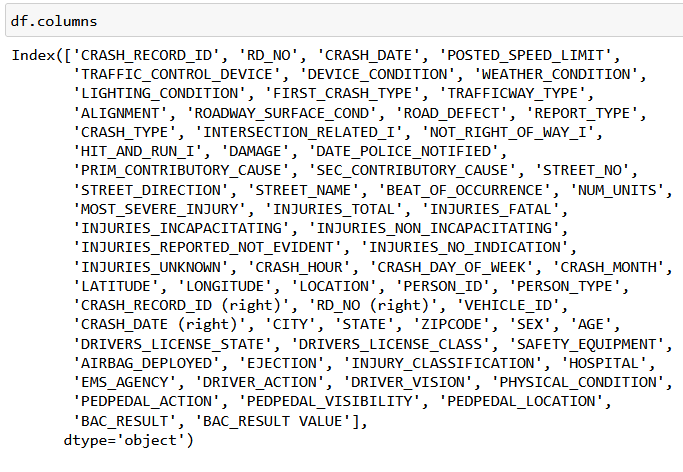
\includegraphics[width=\linewidth]{Chicago_Column.png}
	\caption{Chicago Dataset}
	\label{fig: Chicago Dataset for Crashes and People involved}
 \end{figure}
 \begin{center} 
	\textbf{EDA} 
	\end{center}
Here we show a sampling of some of the attributes classes for the categorical data and numerical.  There are many columns so we will just show a sample of some. You can see more in the code readout. 
\begin{figure}[!h]
	\includegraphics[width=\linewidth]{TOP_DRIVER_PIE.png}
	\caption{Categorical Pie Charts (TOP Driver Reasons)}
	\label{fig: Top Driver Condition Pie chart}
 \end{figure}
More than half of the Top Driver clasifications are not known which hinders our evaluation

\begin{figure}[!h]
	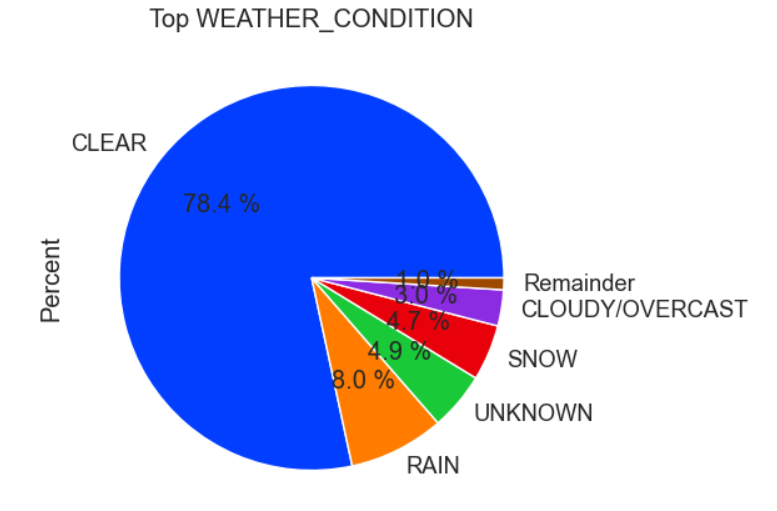
\includegraphics[width=\linewidth]{TOP_WEATHER_CONDITION_PIE.png}
	\caption{Categorical Pie Charts (Sampling View)}
	\label{fig: Top_Weather_Condition Pie chart}
 \end{figure}
Majority of crashes where in clear weather
 
 \begin{figure}[!h]
	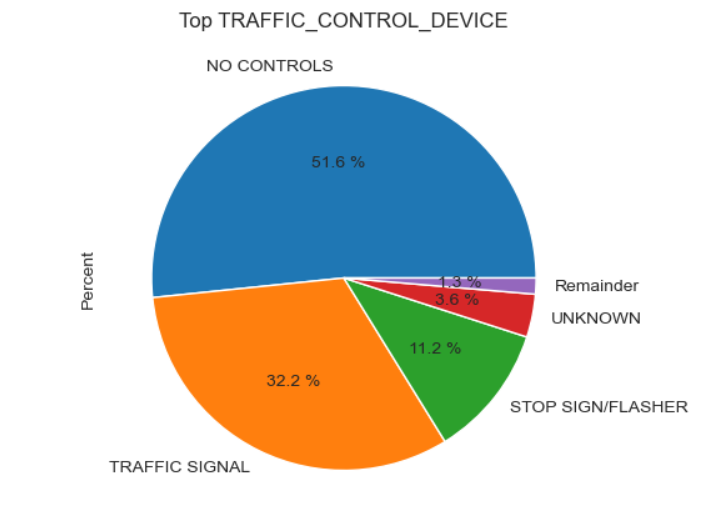
\includegraphics[width=\linewidth]{Traffic_Control_Pie.png}
	\caption{Traffic Control_Pie}
	\label{fig: Traffic_Control_Pie}
 \end{figure}

 Almost 50 percent of crashes had some control place like a stop sign or traffic light

 Here are some of the numeric attributes we examined
 \begin{figure}[!h]
	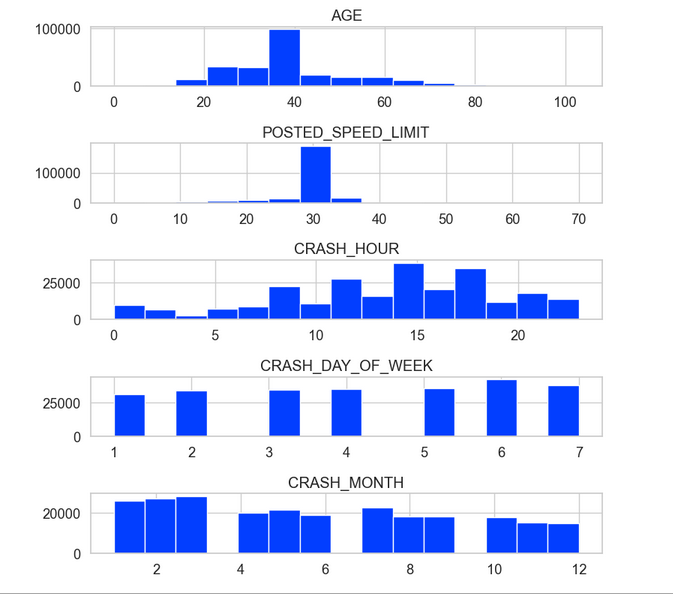
\includegraphics[width=\linewidth]{Numerical_Hist.png}
	\caption{Numeric Histograms (Sampling View)}
	\label{fig: Numeric Histograms}
 \end{figure}

 Couple of callouts for the numerical data is that crashes overindex in the winter months and there is some difference among which of the week seems to matter as well.  Age shows a signficant amount around 39 years old, this seems like a possible data issue but in general the lower the age more likely to have car crash.  Also, the Crash hour chart shows a peak around dinner time which seems like an expected result.

\subsection{Machine Learning Algorithms}
Our data is raw and has no classification or specific purpose so it lends itself to utilize unsupervised data techniques. 
We explored K-modes, kmeans, GMM, kprototype and DBSCAN and will investigate other possible methods to find insights. kprototype is our best hope so far to get good results since it handles both categorical and numeric attributes.  Kmodes can only handle category and kmeans does numerical. We noticed Kprototype takes a very long time to process the model.  Elbow curve took over 24 hours. Since we have a large dataset, training and other tasks take a good length of time for all model types.  We created elbow curves for most of these technique. We'll discuss more in our solution section for each algorithm mentioned

We did some Chi Testing on the attributes to find any that were not relevate but all picked were significant.
\begin{figure}[!h]
	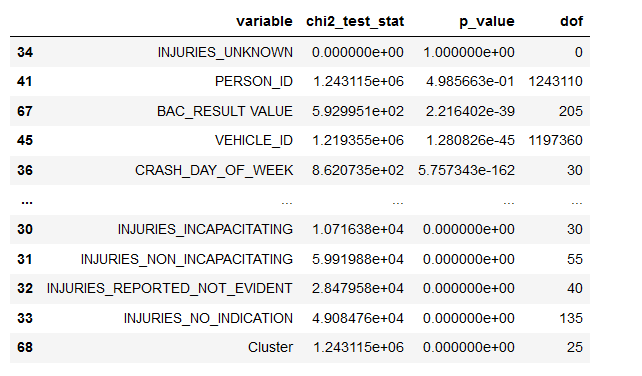
\includegraphics[width=\linewidth]{Chi Square.png}
	\caption{Chi Square Testing View}
	\label{table: Chi Square Testing View}
\end{figure}
We utilized pspark to use groupby by clusters by percent of occurence to see what patterns emerge.  We then exported this view to an excel so we can do further analysis to create a heatmap. We'll look at both the numberical and categorical and for our best solution we describe what each cluster overindexes on compared to the others

\subsection{Implementation Details and Comparison}

 
In this section we'll discuss the results of each method and show more in detail the best solution results.  Figure 9 below shows a summary of the different clustering algorithms.
\begin{figure}[!h]
	\includegraphics[width=\linewidth]{Model_summary.png}
	\caption{Model Summary}
	\label{fig: Model_summary}
\end{figure}

Figure 9 illustrates how each cluster method can be applied.  DBSCAN didn't seem suited for this dataset and it was very difficult to work with in terms of tuning parameters like EPS and Min samples.  Doesn't seem to scale well with all this data.  Kmodes and KPrototype we fairly close but KP had less error with both numberical and categorical combined to the only categorical of the kmodes.  

\begin{center} 
\textbf{Kmodes} 
\end{center}
Kmodes is designed for categorical data only and it a can take the data without hot encoding.  K-modes was successful and did a good job of clustering but you have to take out the numerical data and run that on kmeans.  Therefore it becomes a 2 step process.  The cluster allocation is similar to K-prototype and its error was also one of the lowest in term of SSE.

\begin{figure}[!h]
	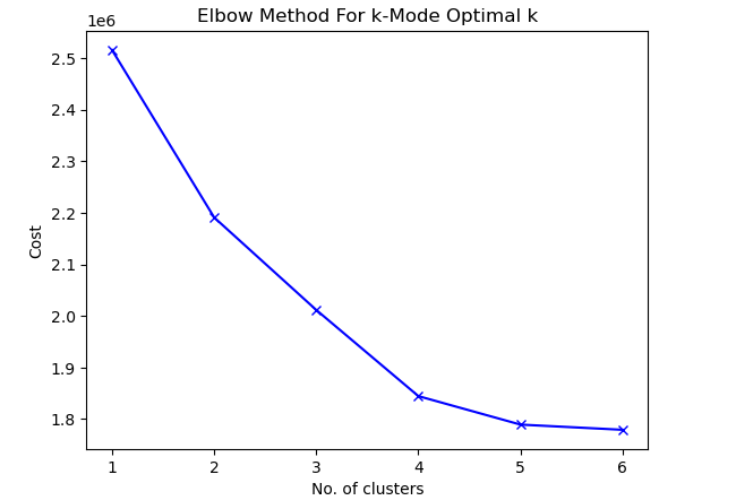
\includegraphics[width=\linewidth]{k_mode_elbow.png}
	\caption{k-mode}
	\label{fig: Kmode Elbow Chart}
 \end{figure}
The elbow chart indicates that 3-4 clusters should be adequate
\begin{figure}[!h]
	\includegraphics[width=\linewidth]{Kmode_Percent_Alloc.png}
	\caption{Kmode Cluster Allocation (Partial View)}
	\label{fig: Kmode Cluster Allocation (Partial View)}
 \end{figure}

 Dark Green represent more allocation vs dark red.  Percent volume of each cluster is reasonable between 20-30 percent.

\begin{center} 
\textbf{Kmeans} 
\end{center}
Kmeans above in the chart reflects the numerical data only,  you can try to run the categorical data with hot encoding but it accuracy or ability to cluster diminishes.

Here is the numerical cluster view,  We used mean and count to assess the numerical data

\begin{figure}[!h]
	\includegraphics[width=\linewidth]{kmeans_num_elbow.png}
	\caption{kmeans}
	\label{fig: Kmeans Elbow Chart}
 \end{figure}
The numerical results were disapointing in that the shared volume across the clusters is similar for larger allocations but there are some minor differences between for the smaller insignificant occurences. Below we show an example for Posted Speed limit allocation for kmeans, you see very little distinction among the clusters.

\begin{figure}[!h]
	\includegraphics[width=\linewidth]{KMEAN_Num_PostedSpeed.png}
	\caption{kmean example for Posted Speed Limit}
	\label{fig: Example View for Kmeans Posted Speed Limit Cluster Allocation}
 \end{figure}

\begin{center} 
\textbf{GMM} 
\end{center}
We used both numeric scaling and hot encoding here but we think that GMM is suited better with only numerical data.  Figure 15 shows the cluster allocation was skewed towards one cluster that has the majority of volume.  This was not our ideal solution.  Here below is partial view of the cluster allocation.  The first cluster is dominate in size with over 69 percent of the population. 
\begin{figure}[!h]
	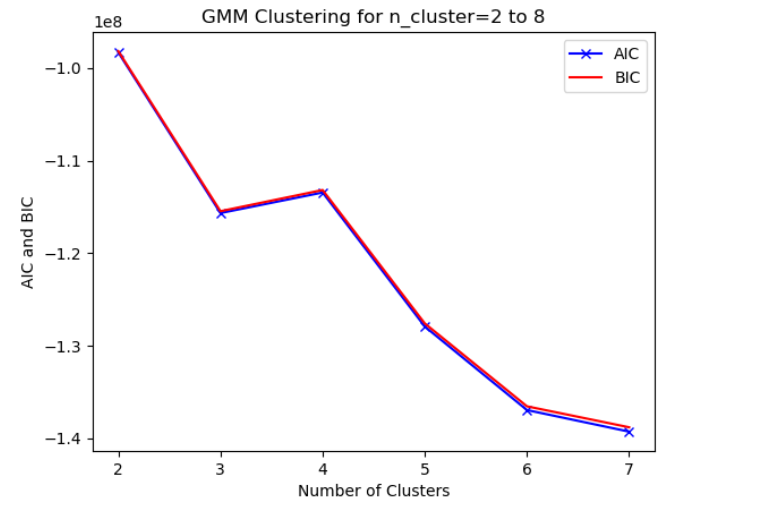
\includegraphics[width=\linewidth]{GMM_Clutering.png}
	\caption{GMM Elbow}
	\label{fig: GMM Elbow}
 \end{figure}
\begin{center}
The AIC and BIC are similar for all cluster values checked

\begin{figure}[!h]
	\includegraphics[width=\linewidth]{GMM_Percent_Results.png}
	\caption{GMM Cluster Results}
	\label{fig: GMM Cluster Results (Partial View)}
 \end{figure}
\begin{center} 

\textbf{DBSCAN} 
\end{center}
DBSCAN was very sensitive to the amount of data and columns.  Only numerical data was used here and finding the EPS and min sample values was a challenge,  Had to iterate through 50 different EPS values to find a sweet spot.  By changing EPS by only 0.01 increments at that sweet spot changed clusters size and number of cluster significantly. The best EPS value for this particular dataset was 28.

\begin{figure}[!h]
	\includegraphics[width=\linewidth]{EP_Finder.png}
	\caption{DBSCAN EPS Finder}
	\label{fig: EPS Finder}
 \end{figure}
We ran category data as well and found it very sensitive to the size of data and number of columns, could not run with the required column size.  Had to reduce the size of the file to get the results below (Show partial view): View in figure 17.

\begin{figure}[!h]
	\includegraphics[width=\linewidth]{DB_Cat.png}
	\caption{DBSCAN Cluster Result}
	\label{fig: DBSCAN Cluster Result}
 \end{figure}
The results were not optimal and we saw again high allocation to one cluster. The -1 or noise cluster had most of the volume,  I spent a consider amount of time to get this result, very sensitive to parameter settings.  We don't think DBSCAN was useful in this application.

\begin{center} 
\textbf{K-prototype} 
\end{center}

K-Prototype was our best soluton in that we can use all the data and train at the same time.  This took significantly longer to train as you can see compared to others in the Comparison table.  The volume allocation was similar to kmodes.  So we can use kmeans for numerical and kmodes for categorical and combine them but KP does it together.  We'll use KP to explain the main difference we see in the 4 clusters we trained on. Also, we did not here of this type of clustering method before and we'll definetly use in the future.
Figure 19 is a partial view of the KP Heatmap for the 4 clusters



 \begin{figure}[!h]
	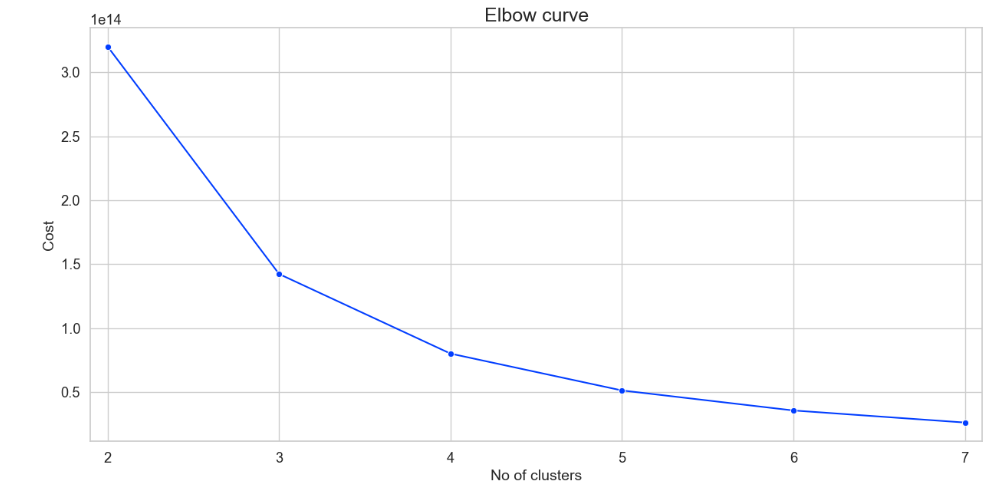
\includegraphics[width=\linewidth]{KPrototype_Elbow.png}
	\caption{k-prototype}
	\label{fig: kprototype elbow chart}
 \end{figure}

\textbf{Cluster-Characteristics} \linebreak

\begin{figure}[!h]
	\includegraphics[width=\linewidth]{Heatmap_KP.png}
	\caption{Example of Cluster Heatmap for Categorical Attributes }
	\label{fig: Cluster Heatmap for Categorical Attributes (4 Clusters)}
\end{figure}


\begin{center} 
	\textbf{Key Cluster Findings} 
	\end{center}
	Cluster 1 \linebreak
	\begin{flushleft}
-In general 1 has the lowest occurrence of crash attributes\linebreak
-lowest occurrence of any crash damage level \linebreak
-Volume is lowest \linebreak
-unlikely for Hit and run cases \linebreak
-first 1-3 day of week occurance \linebreak
	\end{flushleft}

Cluster 2 \linebreak
\begin{flushleft}
-In general 2 has the second lowest occurance of crash attributes \linebreak
-Likely to see Parked Vehicle Crash\linebreak
-likely Hit and Run\linebreak
-overindex on Sex X\linebreak
-overindex on Sex F\linebreak
-first 1-3 day of week occurrence\linebreak
\end{flushleft}

Cluster 3 \linebreak
\begin{flushleft}
-Overindex on Crash Injury \linebreak
-Overindex turning related crash type \linebreak
-Overindex on Interection related crash \linebreak
-Overindex incapaciting injury \linebreak
-Overindex disregarding traffic signals \linebreak
-Overindex device condition functioning properly \linebreak
-Overindex disregarding stop sign \linebreak
-Overindex likely to report on scene \linebreak
-likely to occur in the first 6 months of years \linebreak
\end{flushleft}

Cluster 4 \linebreak
\begin{flushleft}
-Volume is highest \linebreak
-Overindex Parked Motor Vehicle \linebreak
-Overindex on no injury \linebreak
-Overindex no control for device condition (non traffic light) \linebreak
-Overindex to be rear ended \linebreak
-Overindex for follow to closely crash type \linebreak
-Overindex for months 7-12 \linebreak
\end{flushleft}


\begin{figure}[h!]
	% Global parameters for \includegraphics instructions:
	\setkeys{Gin}{height=0.13\textheight,width=0.1\textheight} 
	
	\caption{Comparison of 4 Clusters} % provide a suitable caption
	\bigskip
	\centering
	\begin{tabular}{@{} r @{} *{2}{M{0.13\textheight}} @{}}
	&    cluster 1 and 3 & cluster 2 and 4 \\
	\llap{\quad} & \includegraphics{C1_Heatmap.png} & \includegraphics{C2_Heatmap.png} \\ \addlinespace

	\llap{\quad} & \includegraphics{C3_Heatmap.png} & \includegraphics{C4_Heatmap.png} \\ \addlinespace
 
	\end{tabular}
	\end{figure}

Figure 20 illustrates Cluster distribution by zip.  There are differences among the 4 views. Cluster 1 seems more focused in the south central, cluster 2 focused in south west, Cluster 3 in south east and north and Cluster 4 is more spread out	

\section{Future Directions}
There are Deep Learning techniques that we noticed when we researching other methods but we needed more time to actually pursue it.  One deep learning application was Unsupervised Deep Embedding for Clustering (DEC).  There a need to better evaluate cluster information in terms of what is the cluster characteristics.  A automated evaluation would be useful, we used percent allocation as a meausure but what other methods could be standardized.  There another method for mixed data called Squeezer which can be used with mixed data but has little documentaion.  Deep learning techniques utilizing autoencoders can be examined.  Also, classification of the unsupervised data based on the 4 clusters.  We can then do a multi-nominal logistic regression to better understand how the attributes contribute the most to a particular cluster.  I find that interesting and would like to follow up on this. 
\section{Conclusions}

Cluster analysis is powerful and easily understandable algorithm to utilize in unsupervised applications.  The finding of k-Prototype Algorithm enables to evaluate both numeric and categorical data in one training session.  Learning other methods like DBSCAN, GMM and kmodes was also beneficial to know for future applications.  In terms of the Chicago data, there are some major difference between the clusters and Chicago dept of Transportation may be interested in such analysis to help prevent serious accidents or fix troublesome intersections or poor signing issues. Team learned a lot about the pros and cons of these methods

 
\section{References}
\bibliographystyle{IEEEtran}
\bibliography{}
\begin{flushleft}
1: https://scottmduda.medium.com/categorical-clustering-of-pittsburgh-car-accidents-using-k-modes-7c842cc15d87 
\linebreak
2: https://data.cityofchicago.org/Transportation/Traffic-Crashes-Crashes/85ca-t3if 
\linebreak
3: https://www.freecodecamp.org/news/8-clustering-algorithms-in-machine-learning-that-all-data-scientists-should-know/  
\linebreak
4: https://scikit-learn.org/stable/auto_examples/cluster/plot_dbscan.html 
\linebreak
5: https://antonsruberts.github.io/kproto-audience/ 
\linebreak
6: https://geopandas.org/en/stable/docs/user_guide/mapping.html 
\linebreak


\end{document}


